\baitaptn
\ind{PHẦN I.} \inden{Câu trắc nghiệm nhiều phương án lựa chọn. Mỗi câu hỏi học sinh chỉ chọn một phương án.}\\
\setcounter{ex}{0}
\Opensolutionfile{ans}[ans/0H4-B5-1]

\begin{ex}%[1HK1 - Chuyên Vĩnh Phúc 2019]%[HK1-10-11-Word-T-Begin-lần 2]%[Vũ Công Hoan]%[0H2Y2-1]
	Cho hai vectơ $\overrightarrow{u}=(2;-1),\overrightarrow{v}=(-3;4)$. Tích vô hướng $\overrightarrow{u} \cdot \overrightarrow{v}$ là 
	\choice
	{$11$}
	{\True $-10$}
	{$5$}
	{$-2$}
	\loigiai{
		Ta có $\overrightarrow{u} \cdot \overrightarrow{v}=2 \cdot (-3)+(-1) \cdot 4=-10$.}
\end{ex}

\begin{ex}%[0H2B2-1]
	Cho hai vectơ $\vec{i}$ và $\vec{j}$ vuông góc và có độ dài bằng 1. Xét hai vectơ $\vec{a}=4\vec{i}+6\vec{j}$ và $\vec{b}=3\vec{i}-7\vec{j}$. Tính tích vô hướng $\vec{a}\cdot\vec{b}$.
	\choice
	{$\vec{a}\cdot\vec{b}=30$}
	{$\vec{a}\cdot\vec{b}=43$}
	{$\vec{a}\cdot\vec{b}=3$}
	{\True $\vec{a}\cdot\vec{b}=-30$}
	\loigiai
	{}
\end{ex}

\begin{ex}%[0H2B2-1]
	Trong mặt phẳng $Oxy$, cho ba điểm $A(3;-1 )$, $B(2;10 )$, $C(-4;2 )$. Tính tích vô hướng $\overrightarrow{AB}\cdot\overrightarrow{AC}$.
	\choice
	{$\overrightarrow{AB}\cdot\overrightarrow{AC}=-26$}
	{$\overrightarrow{AB}\cdot\overrightarrow{AC}=26$}
	{$\overrightarrow{AB}\cdot\overrightarrow{AC}=-40$}
	{\True $\overrightarrow{AB}\cdot\overrightarrow{AC}=40$}
	\loigiai
	{Ta có $\overrightarrow{AB}=(-1;11 )$, $\overrightarrow{AC}=(-7;3 )$.
		Suy ra $\overrightarrow{AB}\cdot\overrightarrow{AC}=(-1 )\cdot (-7 )+11\cdot 3=40$. }
\end{ex}


\begin{ex}%[0H2B2-1]
	Trong hệ tọa độ $(O;\overrightarrow{i};\overrightarrow{j} )$, cho vectơ $\overrightarrow{a}=-\dfrac{3}{5}\overrightarrow{i}-\dfrac{4}{5}\overrightarrow{j}$. Độ dài của vectơ $\overrightarrow{a}$ bằng
	\choice
	{$\dfrac{7}{5}$}
	{$\dfrac{1}{5}$}
	{\True $1$}
	{$\dfrac{6}{5}$}
	\loigiai
	{Ta có $\overrightarrow{a}=-\dfrac{3}{5}\overrightarrow{i}-\dfrac{4}{5}\overrightarrow{j}\Rightarrow\overrightarrow{a}=(-\dfrac{3}{5};-\dfrac{4}{5} )\Rightarrow \left| {\overrightarrow{a}} \right|=\sqrt{(-\dfrac{3}{5} )^2+(-\dfrac{4}{5} )^2}=1$. }
\end{ex}

\begin{ex}%[0H2B2-1]
	Trong mặt phẳng $Oxy$, cho hai vectơ $\overrightarrow{a}=(4;3 )$ và $\overrightarrow{b}=(1;7 )$. Tính góc $\alpha $ giữa hai vectơ $\overrightarrow{a}$ và $\overrightarrow{b}$.
	\choice
	{\True $\alpha =45^\circ$}
	{$\alpha =90^\circ$}
	{$\alpha =30^\circ$}
	{$\alpha =60^\circ$}
	\loigiai
	{Ta có $\cos (\overrightarrow{a},\overrightarrow{b} )=\dfrac{\overrightarrow{a}\cdot\overrightarrow{b}}{\left| \overrightarrow{a} \right|\cdot \left| \overrightarrow{b} \right|}=\dfrac{4\cdot 1+3\cdot 7}{\sqrt{16+9}\cdot \sqrt{1+49}}=\dfrac{\sqrt{2}}{2}\Rightarrow(\overrightarrow{a},\overrightarrow{b} )=45^\circ$. }
\end{ex}

\begin{ex}%[0H2B2-1]
	Trong mặt phẳng $Oxy$, cho hai vectơ $\overrightarrow{a}=(-1;1 )$ và $\overrightarrow{b}=(2;0 )$. Tính cosin của góc giữa hai vectơ $\overrightarrow{a}$ và $\overrightarrow{b}$
	\choice
	{$\cos (\overrightarrow{a},\overrightarrow{b} )=\dfrac{1}{\sqrt{2}}$}
	{$\cos (\overrightarrow{a},\overrightarrow{b} )=\dfrac{1}{2}$}
	{\True $\cos (\overrightarrow{a},\overrightarrow{b} )=-\dfrac{\sqrt{2}}{2}$}
	{ $\cos (\overrightarrow{a},\overrightarrow{b} )=-\dfrac{1}{2\sqrt{2}}$}
	\loigiai
	{Ta có $\cos (\overrightarrow{a},\overrightarrow{b} )=\dfrac{\overrightarrow{a}\cdot\overrightarrow{b}}{\left| \overrightarrow{a} \right|\cdot \left| \overrightarrow{b} \right|}=\dfrac{-1\cdot 2+1\cdot 0}{\sqrt{(-1 )^2+1^2}\cdot \sqrt{2^2+0^2}}=-\dfrac{\sqrt{2}}{2}$.}
\end{ex}

\begin{ex}%[0H2B2-1]
	Trong mặt phẳng $Oxy$, cho ba vectơ $\overrightarrow{a}=(1;2 )$, $\overrightarrow{b}=(4;3 )$ và $\overrightarrow{c}=(2;3 )$.
	Tính $P=\overrightarrow{a}\cdot (\overrightarrow{b}+\overrightarrow{c} )$.
	\choice
	{\True $P=18$}
	{$P=28$}
	{$P=0$}
	{$P=20$}
	\loigiai
	{Ta có $\overrightarrow{b}+\overrightarrow{c}=(6;6 )$. Suy ra $P=\overrightarrow{a}\cdot (\overrightarrow{b}+\overrightarrow{c} )=1\cdot 6+2\cdot 6=18$.}
\end{ex}

\begin{ex}%[0H2B2-3]
	Trong mặt phẳng $Oxy$, cho hai vectơ $\overrightarrow{u}=\dfrac{1}{2}\overrightarrow{i}-5\overrightarrow{j}$ và \break $\overrightarrow{v}=k\overrightarrow{i}-4\overrightarrow{j}$. Tìm $k$ để vectơ $\overrightarrow{u}$ vuông góc với $\overrightarrow{v}$.
	\choice
	{$k=-20$}
	{\True $k=-40$}
	{$k=20$}
	{$k=40$}
	\loigiai
	{Từ giả thiết suy ra $\overrightarrow{u}=(\dfrac{1}{2};-5 )$, $\overrightarrow{v}=(k;-4 )$.\\
		Yêu cầu bài toán: $\overrightarrow{u}\perp \overrightarrow{v}\Leftrightarrow \dfrac{1}{2}k+(-5 )(-4 )=0\Leftrightarrow k=-40$.}
\end{ex}

\begin{ex}%[0H2B2-1]
	Trong mặt phẳng $Oxy$, cho hai vectơ $\overrightarrow{u}=\dfrac{1}{2}\overrightarrow{i}-5\overrightarrow{j}$ và \break $\overrightarrow{v}=k\overrightarrow{i}-4\overrightarrow{j}$. Tìm $k$ để vectơ $\overrightarrow{u}$ và vectơ $\overrightarrow{v}$ có độ dài bằng nhau.
	\choice
	{\True $k=\pm \dfrac{\sqrt{37}}{2}$}
	{$k=\dfrac{5}{8}$}
	{$k=\dfrac{37}{4}$}
	{$k=\dfrac{\sqrt{37}}{2}$}
	\loigiai
	{Từ giả thiết suy ra $\overrightarrow{u}=(\dfrac{1}{2};-5 )$, $\overrightarrow{v}=(k;-4 )$.\\
		Suy ra $\left| \overrightarrow{u} \right|=\sqrt{\dfrac{1}{4}+25}=\dfrac{1}{2}\sqrt{101}$ và $\left| \overrightarrow{v} \right|=\sqrt{k^2+16}$. \\
		Do đó để
		$\left| \overrightarrow{u} \right|=\left| \overrightarrow{v} \right|\Leftrightarrow \sqrt{k^2+16}=\dfrac{1}{2}\sqrt{101}\Leftrightarrow k^2+16=\dfrac{101}{4}\Leftrightarrow k^2=\dfrac{37}{4}\Leftrightarrow k=\pm \dfrac{\sqrt{37}}{2}$. }
\end{ex}

\begin{ex}%[0H2B2-1]
	Trong mặt phẳng $Oxy$, tính khoảng cách giữa hai điểm $M(1;-2 )$ và $N(-3;4 )$.
	\choice
	{$MN=3\sqrt{6}$}
	{\True $MN=2\sqrt{13}$}
	{$MN=6$}
	{$MN=4$}
	\loigiai
	{Ta có $\overrightarrow{MN}=(-4;6 )$ suy ra $MN=\sqrt{(-4 )^2+6^2}=\sqrt{42}=2\sqrt{13}$. }
\end{ex}


\begin{ex}%[0H2Y2-1]
	Cho $\vec{a}$ và $\vec{b}$ là hai vectơ cùng hướng và đều khác vectơ $\vec{0}$. Mệnh đề nào sau đây đúng?
	\choice
	{$\vec{a}\cdot\vec{b}=0$}
	{\True $\vec{a}\cdot\vec{b}=\left| \vec{a} \right|\cdot \left| \vec{b} \right|$}
	{$\vec{a}\cdot\vec{b}=-1$}
	{$\vec{a}\cdot\vec{b}=-\left| \vec{a} \right|\cdot\left| \vec{b} \right|$}
	\loigiai
	{Ta có $\vec{a}\cdot\vec{b}=\left| \vec{a} \right|\cdot\left| \vec{b} \right|\cdot\cos(\vec{a},\vec{b} )$.\\
		Do $\vec{a}$ và $\vec{b}$ là hai vectơ cùng hướng nên $(\vec{a},\vec{b} )=0^\circ\Rightarrow\cos(\vec{a},\vec{b} )=1$.
		Vậy $\vec{a}\cdot\vec{b}=\left| \vec{a} \right|\cdot\left| \vec{b} \right|$.}
\end{ex}

\begin{ex}%[0H2B2-1]
	Cho hai vectơ $\vec{a}$ và $\vec{b}$ thỏa mãn $\left| \vec{a} \right|=3$, $\left| \vec{b} \right|=2$ và $\vec{a}\cdot\vec{b}=-3$. Xác định góc $\alpha $ giữa hai vectơ $\vec{a}$ và $\vec{b}$.
	\choice
	{$\alpha =45^\circ$}
	{$\alpha =60^\circ$}
	{\True $\alpha =120^\circ$}
	{$\alpha =30^\circ$}
	\loigiai
	{Ta có $\vec{a}\cdot\vec{b}=\left| \vec{a} \right|\cdot \left| \vec{b} \right|\cdot \cos(\vec{a},\vec{b} )\Rightarrow\cos(\vec{a},\vec{b} )=\dfrac{\vec{a}\cdot\vec{b}}{\left| {\vec{a}} \right|\cdot\left| \vec{b} \right|}=\dfrac{-3}{3\cdot2}=-\dfrac{1}{2}\Rightarrow(\vec{a},\vec{b} )=120^\circ$.}
\end{ex}

\begin{ex}%[0H2B2-1] 
	Cho hai vectơ có độ dài lần lượt là $3$ và $4$ và có tích vô hướng là $-6$. Tính góc giữa hai vectơ đó.
	\choice
	{$60^\circ$}
	{$120^\circ$}
	{\True $45^\circ$}
	{$90^\circ$}
	\loigiai{
		Ta có $\cos \left (\vec{a}, \vec{b}\right ) = \dfrac{\vec{a} \cdot  \vec{b}}{\left |\vec{a}\right | \cdot  \left |\vec{b}\right |} = -\dfrac{1}{2}$. Suy ra  $\left (\vec{a}, \vec{b} \right ) =120^\circ$.
	}
\end{ex}

\begin{ex}%[0H2B2-1]%
	Cho hai vectơ $\overrightarrow{a}$ và $\overrightarrow{b}$ khác $\overrightarrow{0}$. Xác định góc $\alpha $ giữa hai vectơ $\overrightarrow{a}$ và $\overrightarrow{b}$ biết $\overrightarrow{a}\cdot\overrightarrow{b}=-\left| \overrightarrow{a} \right|\cdot\left| \overrightarrow{b} \right|$.
	\choice
	{$\alpha =45^{\circ}$}
	{$\alpha =90^{\circ}$}
	{$\alpha =0^{\circ}$}
	{\True $\alpha =180^{\circ}$}
	\loigiai{
		$\overrightarrow{a}\cdot \overrightarrow{b}=\left| \overrightarrow{a} \right|\cdot \left| \overrightarrow{b} \right|\cdot \cos \alpha $. Mà $\overrightarrow{a}\cdot \overrightarrow{b}=-\left| \overrightarrow{a} \right|\cdot \left| \overrightarrow{b} \right|$, suy ra $\left| \overrightarrow{a} \right|\cdot \left| \overrightarrow{b} \right|\cdot \cos \alpha =-\left| \overrightarrow{a} \right|\cdot \left| \overrightarrow{b} \right|$. Do đó $\cos \alpha =-1$, vì $\alpha$ là góc giữa hai vectơ nên $\alpha =180^{\circ}$.
	}
\end{ex}

\begin{ex}%[0H9H1-6]
	%Câu 12 : 
	Một người dùng một lực $\vec{F}$ có độ lớn là $90$ N làm một vật dịch chuyển một đoạn $100 $ m. Biết lực hợp $\vec{F}$ với hướng dịch chuyển là một góc $60^{\circ}$. Tính công sinh bởi lực $\vec{F}$
	\choice
	{$4500\sqrt{3}(J)$}
	{\True $4500(J)$}
	{$450\sqrt{3}(J)$}
	{$450(J)$}
	\loigiai{
		Công sinh bởi lực $\vec{F}$ được tính bằng công thức
		$$A=\vec{F}\cdot \vec{d}=|\vec{F}|\cdot |\vec{d}|\cdot \cos (\vec{F},\vec{d})=90\cdot 100\cdot \cos 60^\circ=4500 \text{ (J)}.$$
		Vậy công sinh bởi lực $\vec{F}$ có độ lớn bằng $4500$ (J).}
\end{ex}

\begin{ex}%[0H2B2-1]
	\immini[thm]{Tam giác $ ABC$ vuông ở $ A$ và có góc $\widehat B=50^\circ $. Hệ thức nào sau đây {\bf sai}?
		\choice
		{\True $\left(\overrightarrow{AC},\,\overrightarrow{CB}\right)=40^\circ $}
		{$\left(\overrightarrow{AB},\,\overrightarrow{BC}\right)=130^\circ $}
		{$\left(\overrightarrow{BC},\,\overrightarrow{AC}\right)=40^\circ $}
		{$\left(\overrightarrow{AB},\,\overrightarrow{CB}\right)=50^\circ $}}{
		\begin{tikzpicture}[smooth,font=\footnotesize,scale=0.8]
			\path
			(0,0) coordinate (A)
			(4,0) coordinate (B)
			(0,3) coordinate (C);
			\draw (A)--(B)--(C)--cycle
			pic[draw, angle radius=2mm]{right angle=B--A--C};
			\foreach \x/\g in {A/-90,B/-90,C/90} \draw [fill=black] (\x) circle (.05) + (\g:.3) node{$\x$};
	\end{tikzpicture}}
	\loigiai{
		Vì $\left(\overrightarrow{AC},\,\overrightarrow{CB}\right)=180^\circ-\widehat{ACB}=180^\circ-40^\circ=140^\circ $.}
\end{ex}


\begin{ex}%[0H2B2-1]
	\immini[thm]{Cho hình vuông $ABCD$ cạnh $a$.  Tính $\vec{AB}\cdot\vec{AC}$.
		\choice
		{$\vec{AB}\cdot\vec{AC}=a^2\sqrt{2}$}
		{$\vec{AB}\cdot\vec{AC}=\dfrac{\sqrt{2}}{2}a^2$}
		{\True $\vec{AB}\cdot\vec{AC}=a^2$}
		{$\vec{AB}\cdot\vec{AC}=\dfrac{1}{2}a^2$}}{
		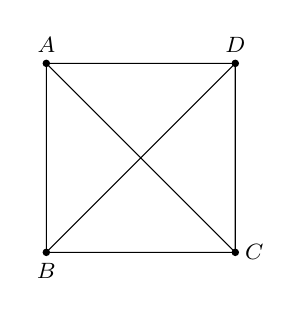
\begin{tikzpicture}[smooth,font=\footnotesize,scale=0.8]
			\path
			(0,3) coordinate (A)
			(0,0) coordinate (B)
			(3,0) coordinate (C)
			(3,3) coordinate (D);
			\draw (A)--(B)--(C)--(D)--cycle (A)--(C) (B)--(D);
			\foreach \x/\g in {A/90,B/-90,C/0,D/90} \draw [fill=black] (\x) circle (.05) + (\g:.3) node{$\x$};
	\end{tikzpicture}	}
	\loigiai
	{Ta có $(\vec{AB},\vec{AC} )=\widehat{BAC}=45^\circ$ nên $\vec{AB}\cdot\vec{AC}=AB\cdot AC\cdot\cos 45^\circ=a\cdot a\sqrt{2}\cdot \dfrac{\sqrt{2}}{2}=a^2$.}
\end{ex}

\begin{ex}%[0H2B2-1]
	Cho tam giác đều $ABC$ có cạnh bằng $a$. Tính tích vô hướng $\vec{AB}\cdot\vec{AC}$.
	\choice
	{$\vec{AB}\cdot\vec{AC}=-\dfrac{a^2\sqrt{3}}{2}$}
	{$\vec{AB}\cdot\vec{AC}=-\dfrac{a^2}{2}$}
	{$\vec{AB}\cdot\vec{AC}=2a^2$}
	{\True $\vec{AB}\cdot\vec{AC}=\dfrac{a^2}{2}$}
	\loigiai
	{Xác định được góc $(\vec{AB},\vec{AC} )$ là góc $\widehat{A}$ nên $(\vec{AB},\vec{AC} )=60^\circ$.\\
		Do đó $\vec{AB}\cdot\vec{AC}=AB\cdot AC\cdot\cos(\vec{AB},\vec{AC} )=a\cdot a\cdot \cos60^\circ=\dfrac{a^2}{2}$.}
\end{ex}


\begin{ex}%[0H2B2-1]%
	Cho tam giác $ABC$ có $AB=5$, $AC=8$, $BC=7$. Tính $\vec{AB}\cdot \vec{AC}$.
	\choice
	{10}
	{$-20$}
	{\True 20}
	{40}
	\loigiai{
		Ta có \begin{eqnarray*}
			&& \vec{BC} = \vec{AC}-\vec{AB}\\
			&\Leftrightarrow & \vec{BC}^2=(\vec{AC}-\vec{AB})^2\\
			&\Leftrightarrow & BC^2=AC^2+AB^2-2\vec{AB}\cdot \vec{AC}\\
			&\Leftrightarrow & \vec{AB}\cdot \vec{AC}=\dfrac{AB^2+AC^2-BC^2}{2}=20.
		\end{eqnarray*}
	}
\end{ex}

\begin{ex}%[0H2B2-1]
	\immini[thm]{Cho hình chữ nhật $ABCD$ có $AB=8$, $AD=5$. Tích $\vec{AB}\cdot\vec{BD}$.
		\choice
		{\True $\vec{AB}\cdot\vec{BD}=-64$}
		{$\vec{AB}\cdot\vec{BD}=64$}
		{$\vec{AB}\cdot\vec{BD}=62$}
		{$\vec{AB}\cdot\vec{BD}=-62$}}{
		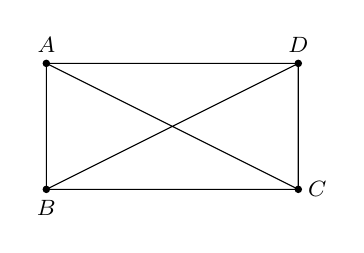
\begin{tikzpicture}[smooth,font=\footnotesize,scale=0.8]
			\path
			(0,2) coordinate (A)
			(0,0) coordinate (B)
			(4,0) coordinate (C)
			(4,2) coordinate (D);
			\draw (A)--(B)--(C)--(D)--cycle (A)--(C) (B)--(D);
			\foreach \x/\g in {A/90,B/-90,C/0,D/90} \draw [fill=black] (\x) circle (.05) + (\g:.3) node{$\x$};
	\end{tikzpicture}}
	\loigiai
	{Ta phân tích các vectơ $\vec{AB}$, $\vec{BD}$ theo các vectơ có giá vuông góc với nhau.\\
		Ta có $$\vec{AB}\cdot\vec{BD}=\vec{AB}\cdot(\vec{BA}+\vec{BC} )=\vec{AB}\cdot\vec{BA}+\vec{AB}\cdot\vec{BC}=-\vec{AB}\cdot\vec{AB}+0=-AB^2=-64.$$}
\end{ex}

\begin{ex}%[DCHT1-Việt Nam-Ba Lan-Hà Nội-19]%[Phan Anh]%[0H2B2-1]
	Trong mặt phẳng tọa độ $Oxy$, cho tam giác $ABC$ có $A(6;0)$, $B(3;1)$, $C(-1;-1)$. Tính số đo góc $B$.
	\choice
	{$\widehat{B}=15^{\circ}$}
	{$\widehat{B}=60^{\circ}$}
	{$\widehat{B}=120^{\circ}$}
	{\True $\widehat{B}=135^{\circ}$}
	\loigiai{Ta có $\overrightarrow{BA}=(3;-1)$, $\overrightarrow{BC}=(-4;-2)$.\\
		Và mặt khác	$\cos B=\cos\left(\overrightarrow{BA},\overrightarrow{BC}\right)=\dfrac{\overrightarrow{BA}\cdot\overrightarrow{BC}}{\left|\overrightarrow{BA}\right|\cdot\left|\overrightarrow{BC}\right|}=\dfrac{-10}{\sqrt{10} \cdot \sqrt{20}}=-\dfrac{\sqrt{2}}{2}$.\\
		Vậy suy ra $\widehat{B}=135^{\circ}$.}
\end{ex}

\begin{ex}%[DCHT1-Việt Nam-Ba Lan-Hà Nội-19]%[Phan Anh]%[0H2B2-1]
	Trong mặt phẳng tọa độ $Oxy$, cho tam giác $ABC$ có $A(1;4)$, $B(3;2)$, $C(5;4)$. Tính chu vi $P$ của tam giác đã cho.
	\choice
	{$P=4+2\sqrt{2}$}
	{\True $P=4+4\sqrt{2}$}
	{$P=8+8\sqrt{2}$}
	{$P=2+2\sqrt{2}$}
	\loigiai{Ta có $\overrightarrow{AB}=(2;-2)\Rightarrow AB=2\sqrt{2}$, $\overrightarrow{BC}=(2;2)\Rightarrow BC=2\sqrt{2}$, $\overrightarrow{AC}=(4;0)\Rightarrow AC=4$.\\
		Vậy nên chu vi của tam giác $ABC$ là $P=AB+BC+AC=4+4\sqrt{2}$.}
\end{ex}

\begin{ex}%[0H2B2-4]
	Trong mặt phẳng tọa độ $Oxy$, cho hai điểm $A(2;2 ),B(5;-2 )$.  Tìm điểm $M$ thuộc trục hoành sao cho $\widehat{AMB}=90^\circ$.
	\choice
	{$M(1;6 )$}
	{\True $M(6;0 )$}
	{$M(0;6 )$}
	{$M(0;1 )$}
	\loigiai
	{Ta có $M\in Ox$ nên $M(m;0 )$ và $\heva{
			& \overrightarrow{AM}=(m-2;-2) \\
			& \overrightarrow{BM}=(m-5;2 ) \\
		}$.
		Vì $\widehat{AMB}=90^\circ$ suy ra $\overrightarrow{AM}\cdot\overrightarrow{BM}=0$ nên $(m-2 )(m-5 )+(-2 )\cdot2=0$.
		$\Leftrightarrow m^2-7m+6=0\Leftrightarrow \hoac{
			& m=1 \\
			& m=6 \\
		} \Rightarrow\hoac{
			& M(1;0 ) \\
			& M(6;0 ) \\
		}$. }
\end{ex}

\begin{ex}%[0H2K2-4]
	Trong mặt phẳng tọa độ $Oxy$, cho tam giác $ABC$ có $A(-4;1 )$, $B(2;4 )$, $C(2;-2 )$. Tìm tọa độ tâm $I$ của đường tròn ngoại tiếp tam giác đã cho.
	\choice
	{$I\left(\dfrac{1}{4};1 \right)$}
	{$I\left(1;\dfrac{1}{4} \right)$}
	{\True $I\left(-\dfrac{1}{4};1 \right)$}
	{$I\left(1;-\dfrac{1}{4} \right)$}
	\loigiai
	{Gọi $I(x;y )$. Ta có $\heva{
			& \overrightarrow{AI}=(x+4;y-1 ) \\
			& \overrightarrow{BI}=(x-2;y-4 ) \\
			& \overrightarrow{CI}=(x-2;y+2 ) \\
		}$. \\
		Do $I$ là tâm đường tròn ngoại tiếp tam giác $ABC$ nên \begin{eqnarray*}
			IA=IB=IC&\Leftrightarrow& \left\{ \begin{aligned}
				&IA^2=IB^2 \\
				&IB^2=Ic^2 \\
			\end{aligned} \right.\\
			&\Leftrightarrow& \left\{ \begin{aligned}
				&{{(x+4 )}^2}+{{(y-1 )}^2}={{(x-2 )}^2}+{{(y-4 )}^2} \\
				&{{(x-2 )}^2}+{{(y-4 )}^2}={{(x-2 )}^2}+{{(y+2 )}^2} \\
			\end{aligned} \right.\Leftrightarrow \left\{ \begin{aligned}
				&{{(x+4 )}^2}={{(x-2 )}^2}+9 \\
				&y=1 \\
			\end{aligned} \right.\\
			&\Leftrightarrow& \left\{ \begin{aligned}
				&x=-\dfrac{1}{4} \\
				&y=1. \\
			\end{aligned} \right.
	\end{eqnarray*}}
\end{ex}

%C:\Users\Admin\Desktop\rrrr.tex
\begin{ex}%[0H2K2-4]
	Trong mặt phẳng tọa độ $Oxy$, cho tam giác $ABC$ có $A(-3;0 )$, $B(3;0 )$ và $C(2;6 )$. Gọi $H(a;b )$ là tọa độ trực tâm của tam giác đã cho. Tính $a+6b$.
	\choice
	{\True $a+6b=7$}
	{$a+6b=6$}
	{$a+6b=5$}
	{$a+6b=8$}
	\loigiai
	{Ta có $\heva{
			& \overrightarrow{AH}=(a+3;b )\\
			& \overrightarrow{BC}=(-1;6 ) \\
			& \overrightarrow{BH}=(a-3;b )\\
			& \overrightarrow{AC}=(5;6 ) \\
		}$.  \\
		Từ giả thiết, ta có:
		$\heva{
			& \overrightarrow{AH}\cdot\overrightarrow{BC}=0 \\
			& \overrightarrow{BH}\cdot\overrightarrow{AC}=0 \\
		}$ $\Leftrightarrow \heva{
			& (a+3 )\cdot (-1 )+b.6=0 \\
			& (a-3 )\cdot 5+b.6=0 \\
		} $ $\Leftrightarrow \heva{
			& a=2 \\
			& b=\dfrac{5}{6} \\
		} \Rightarrow a+6b=7$. }
\end{ex}

\Closesolutionfile{ans}

\ind{PHẦN II.} \inden{Câu trắc nghiệm đúng sai. Trong mỗi ý a), b), c), d) ở mỗi câu, học sinh chọn đúng hoặc sai.}\\
\Opensolutionfile{ans}[ans/0H4-B5-2]

\begin{ex}%[0H2B2-1]
	Trong mặt phẳng $Oxy$, cho hai vectơ $\vec{a}=4\vec{i}+3\vec{j}$ và $\vec{b}=\vec{i}+7\vec{j}$. Xét tính đúng sai của các khẳng định sau:
	\choiceTF
	{$\big|\vec{a}\big|=7$}
	{\True $\big|\vec{b}\big|=5\sqrt{2}$}
	{$\vec{a} \cdot \vec{b}=14$}
	{\True $\big(\vec{a},\vec{b}\big)=45^\circ$}
	\loigiai{
		Ta cso $\vec{a}=(4;3)$, $\vec{ab}=(1;7)$
		\begin{itemchoice}
			\itemch $\big|\vec{a}\big|=\sqrt{4^2+3^2}=5$.
			\itemch $\big|\vec{b}\big|\sqrt{41^2+7^2}=5\sqrt{2}$
			\itemch $\vec{a} \cdot \vec{b}=4.1+3.7=25$
			\itemch $\cos\left(\vec{a},\vec{b} \right)=\dfrac{\vec{a} \cdot \vec{b}}{\big|\vec{a}\big|\cdot \big|\vec{b}\big|}=\dfrac{\sqrt{2}}{2}\Rightarrow \big(\vec{a},\vec{b}\big)=45^\circ$.
		\end{itemchoice}
	}
\end{ex}

\begin{ex}
	Cho tam giác $ABC$ vuông tại $A$, có số đo góc $B$ là $60^{\circ}$ và $AB=a$. Xét tính đúng sai của các khẳng định sau:
	\choiceTF
	{$\overrightarrow{AC}\cdot \overrightarrow{CB}=-3\sqrt{2} a$}
	{\True$\overrightarrow{AB}\cdot \overrightarrow{AC}=0$}
	{\True$\overrightarrow{CA}\cdot \overrightarrow{CB}=3 a^2$}
	{\True$\overrightarrow{AB}\cdot \overrightarrow{BC}=-a^2$}
\loigiai{
	Xét tam giác $ABC$ vuông tại $A$ có $\widehat{B} = 60^\circ$ và $AB = a$, ta tính được các cạnh và góc còn lại:
	\begin{itemize}
		\item $AC = AB \cdot \tan 60^\circ = a\sqrt{3}$.
		\item $BC = \dfrac{AB}{\cos 60^\circ} = \dfrac{a}{\dfrac{1}{2}} = 2a$.
		\item $\widehat{C} = 90^\circ - \widehat{B} = 30^\circ$.
	\end{itemize}
	Ta đi xét tính đúng sai của từng khẳng định:
	\begin{enumerate}[a)]
		\item Xét $\overrightarrow{AC} \cdot \overrightarrow{CB}$:\\
		Ta có $\overrightarrow{AC} \cdot \overrightarrow{CB} = -\overrightarrow{CA} \cdot \overrightarrow{CB} = - \left|\overrightarrow{CA}\right| \cdot \left|\overrightarrow{CB}\right| \cdot \cos\left(\overrightarrow{CA}, \overrightarrow{CB}\right)$.\\
		Góc giữa hai vectơ $\overrightarrow{CA}$ và $\overrightarrow{CB}$ chính là góc $\widehat{C} = 30^\circ$.\\
		Suy ra: $\overrightarrow{AC} \cdot \overrightarrow{CB} = - (a\sqrt{3}) \cdot (2a) \cdot \cos 30^\circ = -2\sqrt{3}a^2 \cdot \dfrac{\sqrt{3}}{2} = -3a^2$.\\
		Do $-3a^2 \neq -3\sqrt{2}a$, nên khẳng định a) là \textbf{Sai}.
		
		\item Xét $\overrightarrow{AB} \cdot \overrightarrow{AC}$:\\
		Vì tam giác $ABC$ vuông tại $A$ nên $AB \perp AC$, do đó $\overrightarrow{AB} \cdot \overrightarrow{AC} = 0$.\\
		Khẳng định b) là \textbf{Đúng}.
		
		\item Xét $\overrightarrow{CA} \cdot \overrightarrow{CB}$:\\
		Ta có $\overrightarrow{CA} \cdot \overrightarrow{CB} = \left|\overrightarrow{CA}\right| \cdot \left|\overrightarrow{CB}\right| \cdot \cos\widehat{C} = (a\sqrt{3}) \cdot (2a) \cdot \cos 30^\circ = 2\sqrt{3}a^2 \cdot \dfrac{\sqrt{3}}{2} = 3a^2$.\\
		Khẳng định c) là \textbf{Đúng}.
		
		\item Xét $\overrightarrow{AB} \cdot \overrightarrow{BC}$:\\
		Ta có $\overrightarrow{AB} \cdot \overrightarrow{BC} = -\overrightarrow{BA} \cdot \overrightarrow{BC} = - \left|\overrightarrow{BA}\right| \cdot \left|\overrightarrow{BC}\right| \cdot \cos\widehat{B}$.\\
		Suy ra: $\overrightarrow{AB} \cdot \overrightarrow{BC} = - a \cdot 2a \cdot \cos 60^\circ = -2a^2 \cdot \dfrac{1}{2} = -a^2$.\\
		Khẳng định d) là \textbf{Đúng}.
	\end{enumerate}
}
\end{ex}

\begin{ex}%[0H5N4-1]
	%Câu 1: 
	Cho hình vuông $ABCD$ có cạnh bằng $a$. Xét tính đúng sai của các khẳng định sau:
	\choiceTF
	{\True  $\overrightarrow{AC}\cdot \overrightarrow{BD}=0$}
	{$\left( \overrightarrow{AC},\overrightarrow{BC} \right)=135^{\circ}$}
	{\True  $\overrightarrow{AB}\cdot \overrightarrow{AC}=a^2$}
	{$\overrightarrow{AB}\cdot \overrightarrow{BD}=-\dfrac{a^2}{2}$}
	\loigiai{
		\begin{itemchoice}
			\itemch   Vì $\left( \overrightarrow{AC},\overrightarrow{BD} \right)=90^{\circ}$ nên $\overrightarrow{AC}\cdot \overrightarrow{BD}=0$. Vậy mệnh đề đúng.
			\itemch  $\left( \overrightarrow{AC},\overrightarrow{BC} \right)=\left( \overrightarrow{AC},\overrightarrow{AD} \right)=\widehat{CAD}=45^{\circ}$. Vậy mệnh đề sai.
			\itemch $\overrightarrow{AB}\cdot \overrightarrow{AC}=AB\cdot AC\cdot \cos \left( \overrightarrow{AB},\overrightarrow{AC} \right)=a\cdot a\sqrt{2}\cdot \cos 45^{\circ} =a\cdot a\sqrt{2}\cdot \dfrac{\sqrt{2}}{2}=a^2$.
			Mệnh đề đúng.
			\itemch  $\overrightarrow{AB}\cdot \overrightarrow{BD}=AB\cdot BD\cdot \cos \left( \overrightarrow{AB},\overrightarrow{BD} \right)=a\cdot a\sqrt{2}\cdot \cos 135^{\circ}=a\cdot a\sqrt{2}\cdot \left( -\dfrac{\sqrt{2}}{2} \right)=-a^2$.
			Mệnh đề sai.
		\end{itemchoice}
	}
\end{ex}

\begin{ex}%[0H5N4-1]
	%Câu 3: 
	Cho tam giác đều $ABC$ tâm $O$, có độ dài các cạnh bằng $a$. Xét tính đúng sai của các khẳng định sau:
	\choiceTF
	{\True Góc giữa vectơ $\overrightarrow{AB}$ và $\overrightarrow{AC}$ bằng $60^{\circ}$}
	{Góc giữa vectơ $\overrightarrow{AB}$ và $\overrightarrow{BC}$ bằng $60^{\circ}$}
	{\True Tích vô hướng của $\overrightarrow{OA}$ và $\overrightarrow{BC}$ bằng $0$}
	{Tích vô hướng của $\overrightarrow{OA}$ và $\overrightarrow{OB}$ bằng $-\dfrac{a^2}{2}$}
	\loigiai{
		\immini{\begin{itemchoice}
				\itemch $\left( \overrightarrow{AB},\overrightarrow{AC} \right)=\widehat{BAC}=60^{\circ}$ nên mệnh đề đúng.
				\itemch $\left( \overrightarrow{AB},\overrightarrow{AC} \right)=180^{\circ}-\widehat{ABC}=180^{\circ}-60^\circ =120^{\circ}$ nên mệnh đề sai.
				\itemch Do $\overrightarrow{OA}\perp \overrightarrow{BC}\Rightarrow \overrightarrow{OA}\cdot \overrightarrow{BC}=0$ nên mệnh đề đúng.
				\itemch Ta có $\overrightarrow{OA}\cdot \overrightarrow{OB}=\left| \overrightarrow{OA} \right|\cdot \left| \overrightarrow{OB} \right|\cdot \cos \left( \overrightarrow{OA},\overrightarrow{OB} \right)$,\\
				$+\left( \overrightarrow{OA},\overrightarrow{OB} \right)=\widehat{AOB}=180^{\circ}-2\cdot 30^{\circ}=120^{\circ}.$	 \\
				$+\left| \overrightarrow{OA} \right|=\left| \overrightarrow{OB} \right|=\dfrac{2}{3}\cdot \dfrac{a\sqrt{3}}{2}=\dfrac{a\sqrt{3}}{3}.$\\
				Vậy $\overrightarrow{OA}\cdot \overrightarrow{OB}=\left( \dfrac{a\sqrt{3}}{3} \right)^2\cdot \cos 120^0=-\dfrac{a^2}{6}$ nên mệnh đề sai.
		\end{itemchoice}}
		{\begin{tikzpicture}[scale=0.8, font=\footnotesize, line join=round, line cap=round, >=stealth]
				\path	(0,0) coordinate (B)
				(4,0) coordinate (C)
				($(B)!1!60:(C)$) coordinate (A)
				($(B)!1/2!(C)$)coordinate (M)
				($(A)!1/2!(C)$)coordinate (N)
				($(A)!2/3!(M)$)coordinate (O)
				;
				\draw (A)--(B)--(C)--cycle (A)--(M) (B)--(N);
				\foreach \x/\g in {A/90,B/-90,C/-90,O/-40}  \fill (\x) circle (1.2pt)+(\g:.3)node {$\x$};	
		\end{tikzpicture}}
	}
\end{ex}

\Closesolutionfile{ans}

\ind{PHẦN III.} \inden{Câu trắc nghiệm trả lời ngắn.}\\
\Opensolutionfile{ans}[ans/0H4-B5-3]
\begin{ex}%[0H2B2-3]
	Trong mặt phẳng $Oxy$, cho $\vec{u}=\dfrac{1}{2}\vec{i}-5\vec{j}$ và $\vec{v}=k\vec{i}-4\vec{j}$. Tìm $k$ để vectơ $\vec{u}$ vuông góc với $\vec{v}$.\\
	\shortans[oly]{$-40$}
	\loigiai
	{Từ giả thiết suy ra $\vec{u}=(\dfrac{1}{2};-5 )$, $\vec{v}=(k;-4 )$.\\
		Yêu cầu bài toán: $\vec{u}\perp \vec{v}\Leftrightarrow \dfrac{1}{2}k+(-5 )(-4 )=0\Leftrightarrow k=-40$.}
\end{ex}

\begin{ex}%[0H2B2-1] 
	\immini[thm]{Tính công sinh bởi một lực $\vec{F}$ có độ lớn $60$ N kéo một vật di chuyển một vectơ $\vec{d}$ có độ dài $200$ m. Cho biết $(\vec{F},\vec{d})=60^\circ$.\\
		\shortans[oly]{$6000$}
	}{\hspace{1cm}
		\begin{tikzpicture}[smooth,font=\footnotesize,scale=0.5,>=latex]
			\path
			(0,0) coordinate (A)
			(3,0) coordinate (B)
			(3,2) coordinate (C)
			(0,2) coordinate (D)
			(3,0.7) coordinate (O)
			(10,0.7) coordinate (M)
			(5,4.5) coordinate (N);
			\fill[cyan] (A)--(B)--(C)--(D)--cycle;
			\draw (A)--(B)--(C)--(D)--cycle
			pic["$60^\circ$",angle radius=14mm,blue]{angle=M--O--N}
			pic[draw, angle radius=5mm,blue]{angle=M--O--N};
			\draw[->,thick,magenta] (O)--(M)node[below left]{$\vec{d}$};
			\draw[->,thick,magenta] (O)--(N)node[right]{$\vec{F}$};
	\end{tikzpicture}}
	\loigiai{
		Ta có $A=\vec{F}\cdot \vec{d}=|\vec{F}|\cdot |\vec{d}|\cdot \cos(\vec{F},\vec{d})=60\cdot 200\cdot \cos 60^\circ=60\cdot 200\cdot \dfrac{1}{2}=6000$ J.
	}
\end{ex}

\begin{ex}%[0H5B4-2]
	Trong mặt phẳng toạ độ $Oxy$, cho tam giác $ABC$, biết $A(2;-2)$, $B(3;-4)$, $C(0;-8)$. Góc $A$ của tam giác bằng bao nhiêu độ?\\
	\shortans[oly]{$45$}
	\loigiai{
		Ta có $\widehat{BAC}=\left(\overrightarrow{AB},\overrightarrow{AC}\right)$, 
		$\overrightarrow{AB}=(1;-2)$, $\overrightarrow{AC}=(-2;-6)$.\\
		$\Rightarrow \cos\left(\overrightarrow{AB},\overrightarrow{AC}\right)=\dfrac{\overrightarrow{AB}.\overrightarrow{AC}}{\left|\overrightarrow{AB}\right|\cdot \left|\overrightarrow{AC}\right|}=\dfrac{1\cdot (-2)+(-2)\cdot (-6)}{\sqrt{1^2+(-2)^2}\cdot \sqrt{(-2)^2+(-6)^2}}=\dfrac{\sqrt{2}}{2}$.\\
		$\Rightarrow \widehat{BAC}=\left(\overrightarrow{AB},\overrightarrow{AC}\right)=45^\circ$.
	}
\end{ex}

\begin{ex}%[WTT-1234 câu TN10, Trần Minh]%[0H2B2-1]%
	Cho tam giác $ABC$ đều cạnh bằng $4$, trọng tâm $G$. Tính $\overrightarrow{BC}\cdot \overrightarrow{CG}$.\\
	\shortans[oly]{$-8$}
	\loigiai{
		\immini
		{
			Ta có \\
			$\begin{aligned}
				\overrightarrow{BC}\cdot \overrightarrow{CG}&=\left|\overrightarrow{BC}\right|\cdot \left|\overrightarrow{CG}\right|\cdot \cos \left(\overrightarrow{BC},\overrightarrow{CG}\right)\\
				&=BC\cdot CG\cdot \cos \left(\overrightarrow{CB'},\overrightarrow{CG}\right)\\
				&=BC\cdot CG\cdot \cos 150^{\circ}\\
				&=a\cdot \dfrac{2}{3}\cdot \dfrac{a\sqrt{3}}{2}\cdot \left(-\dfrac{\sqrt{3}}{2}\right)\\
				&=-\dfrac{a^2}{2}.
			\end{aligned}$
		}
		{
			\begin{tikzpicture}[scale=1, font=\footnotesize, line join = round, line cap = round,>=stealth]
				\tkzDefPoints{0/0/G,0/2/A,0/-1/I}
				\coordinate (C) at ($(G)+({2*cos(-30)},{2*sin(-30)})$);
				\coordinate (B) at ($(G)+({2*cos(-150)},{2*sin(-150)})$);
				\coordinate (B') at ($(B)!2!(C)$);
				\tkzDrawPoints[fill=black](A,B,C,G,B')
				\tkzDrawSegments(A,I A,B A,C)
				\tkzLabelPoints[below](B,C,B')
				\tkzLabelPoints[left](G)
				\tkzLabelPoints[above](A)
				\tkzDrawSegments[->](C,G B,C C,B')
				\tkzMarkAngles[size=0.2cm,arc=l](B',C,G)
			\end{tikzpicture}
		}
	}
\end{ex}

\begin{ex}%[0H2B2-1]
	\immini[thm]{Cho hình thoi $ABCD$ có $AC=8$ và $BD=6$. Tính $\vec{AB}\cdot\vec{AC}$. \\
		\shortans[oly]{$32$}
	}{
		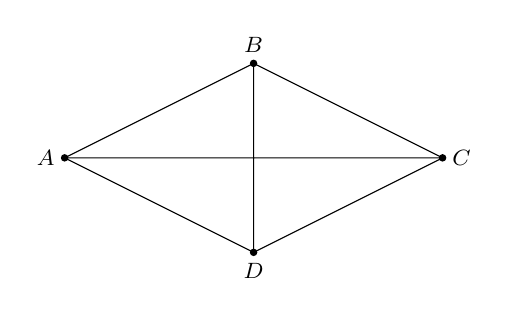
\begin{tikzpicture}[smooth,font=\footnotesize,scale=0.8]
			\path
			(0,0) coordinate (A)
			(6,0) coordinate (C)
			(3,1.5) coordinate (B)
			(3,-1.5) coordinate (D);
			\draw (A)--(B)--(C)--(D)--cycle (B)--(D) (A)--(C)
			;
			\foreach \x/\g in {A/180,B/90,C/0,D/-90} \draw [fill=black] (\x) circle (.05) + (\g:.3) node{$\x$};
	\end{tikzpicture}}
	\loigiai
	{		\immini{Gọi $O=AC\cap BD$, giả thiết không cho góc, ta phân tích các vectơ $\vec{AB},\vec{AC}$ theo các vectơ có giá vuông góc với nhau.\\
			Ta có \begin{eqnarray*}
				\vec{AB}\cdot\vec{AC}&=&(\vec{AO}+\vec{OB} )\cdot\vec{AC}\\
				&=&\vec{AO}\cdot\vec{AC}+\vec{OB}\cdot\vec{AC}\\
				&=&\dfrac{1}{2}\vec{AC}\cdot\vec{AC}+0=\dfrac{1}{2}AC^2=32.
		\end{eqnarray*}}{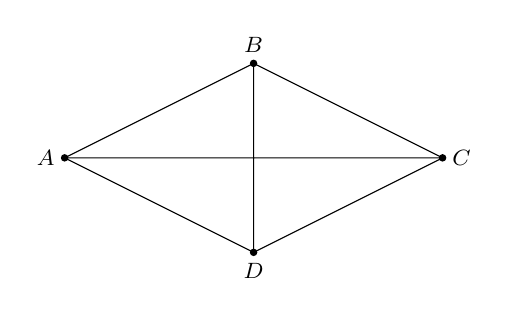
\begin{tikzpicture}[smooth,font=\footnotesize,scale=0.8]
				\path
				(0,0) coordinate (A)
				(6,0) coordinate (C)
				(3,1.5) coordinate (B)
				(3,-1.5) coordinate (D);
				\draw (A)--(B)--(C)--(D)--cycle (B)--(D) (A)--(C)
				;
				\foreach \x/\g in {A/180,B/90,C/0,D/-90} \draw [fill=black] (\x) circle (.05) + (\g:.3) node{$\x$};
		\end{tikzpicture}}
	}
\end{ex}

\begin{ex}%[0H2B2-1]
	\immini[thm]{Cho hình bình hành $ABCD$ có $AB=8$ cm, $AD=12$ cm, góc $\widehat{ABC}$ nhọn và diện tích bằng $54$ cm$^2$. Tính $\cos (\vec{AB},\vec{BC} )$ (kết quả làm tròn đến 1 chữ số thập phân). \\
		\shortans[oly]{$-0,8$}
	}{
		\begin{tikzpicture}[scale=0.8]
			\tkzDefPoints{0/0/B,4/0/C,1/2/A}
			\coordinate (D) at ($(A)+(C)-(B)$);
			\tkzDrawPoints[fill=black](A,B,C,D)
			\tkzDrawSegments(A,B B,C C,D D,A)
			\tkzLabelPoints[above](A,D)\tkzLabelPoints[below](C,B)
	\end{tikzpicture}}
	\loigiai
	{
		\immini{Ta có $S_{ABCD}=2\cdot S_{\triangle ABC}=54\Leftrightarrow S_{\triangle ABC}=27$ cm$^2$. \\
			Diện tích tam giác $ABC$ là:
			$$S_{\triangle ABC}=\dfrac{1}{2}\cdot AB\cdot BC\cdot \sin \widehat{ABC}=\dfrac{1}{2}\cdot AB\cdot AD\cdot\sin \widehat{ABC}.$$}{\begin{tikzpicture}[scale=0.6]
				\tkzDefPoints{0/0/B,4/0/C,1/2/A}
				\coordinate (D) at ($(A)+(C)-(B)$);
				\tkzDrawPoints[fill=black](A,B,C,D)
				\tkzDrawSegments(A,B B,C C,D D,A)
				\tkzLabelPoints[above](A,D)\tkzLabelPoints[below](C,B)
		\end{tikzpicture}}
		\noindent $\Rightarrow \sin \widehat{ABC}=\dfrac{2\cdot S_{\triangle ABC}}{AB\cdot AD}=\dfrac{2\cdot 27}{8\cdot 12}=\dfrac{9}{16}$
		$\Rightarrow\cos \widehat{ABC}=\sqrt{1-\sin ^2\widehat{ABC}}=\dfrac{5\sqrt{7}}{16}$(vì $\widehat{ABC}$ nhọn).\\
		Mặt khác góc giữa hai vectơ $\vec{AB}$, $\vec{BC}$ là góc ngoài của góc $\widehat{ABC}$.\\
		Suy ra $\cos (\vec{AB},\vec{BC} )=\cos (180^\circ-\widehat{ABC} )=-\cos \widehat{ABC}=-\dfrac{5\sqrt{7}}{16}$. 
	}
\end{ex}

\Closesolutionfile{ans}
